
\subsection{Tested Propreties}
In this section, we will give and explain the code to formally verify that our system is correct. We are going to check :
\begin{itemize}
	\item Safety : unwanted system states are never reached (e.g. conflicting green light),
	\item Liveness : desired behavior eventually happen (e.g. everyone get a green light at some point),
	\item Fairness : infinitely done requests are infinitely satisfied (nobody will have to wait too long).
\end{itemize}

The first two have been checked with Uppaal and the last one with Prism.

\subsubsection{Liveness}
We will first give some liveness properties about our system.
\begin{enumerate}
  \item If a bus has been called, he will never have to wait indefinitely to cross the road. Since our bus can reach several states, we check for each of them if the light will be green at some point. 
  \begin{itemize}
    \item $Bus.DelayedCall --> Bus.Green$ 
    \item $Bus.Preempted --> Bus.Green$
    \item $Bus.Called --> Bus.Green$
  \end{itemize}
  \item If a pedestrian call has been made, they will never have to wait indefinitely to cross the crosswalk. Since our pedestrians can reach several states, we check for each of them if the light will be green at some point. 
  \begin{itemize}
    \item $Crosswalk.DelayedCall --> Crosswalk.Green$ 
    \item $Crosswalk.Preempted --> Crosswalk.Green$
    \item $Crosswalk.Called --> Crosswalk.Green$
  \end{itemize}
  \item No deadlock, meaning that the system will never freeze.
  \begin{itemize}
    \item \textit{A[] not deadlock}
  \end{itemize}
\end{enumerate}
Since we use Uppaal TiGa, there is not only a controller but also an environment. We thus took this into consideration and we wrote some properties about the maximum time one actor of the environment will have to wait.
\begin{enumerate}
  \item The maximum waiting time for a pedestrian is at most 3P (meaning 3 times the period we have chosen). Indeed, if he has just been called recently, he will have to wait 2P and if a bus has been called before, we have to give him the priority and wait 1P.
  \begin{itemize}
    \item \textit{A[] not( Crosswalk.Green \&\& Crosswalk.ct>4*P)}
    \item We here have to put 4P because the light will stay green until the end of the fourth green light
  \end{itemize}
  \item The maximum waiting time for a bus is at most 2P. Indeed, if he has just been called recently, he will have to wait 2P since the bus has the priority.
  \begin{itemize}
    \item \textit{A[] not( Bus.Green \&\& Bus.bt>3*P )}
    \item We here have to put 3P because the light will stay green until the end of the third green light
  \end{itemize}
  \item The cars traffich lights will be green again before 4P.
  \begin{itemize}
    \item \textit{A[] not( TrafficLightFrontBack.Green \&\& TrafficLightFrontBack.tlfbc>4*P )}
    \item \textit{A[] not( TrafficLightLeftRight.Green \&\& TrafficLightLeftRight.tllrc>4*P )}
  \end{itemize}
\end{enumerate}
\subsubsection{Safety} 
On the opposite of the first proprety we defined, the liveness one, we will here not try to find that something willeventually happen. We will here show that some events will \textbf{never} happen because if it was the case, we would reach incoherent states leading to a failure in our system. In our traffic light model, it would means that two opposite actors could cross the crossroad at the same time, leading to a crash. 
\begin{enumerate}
  \item We check that if the crosswalk light is green, no other lights can be green at the same time.
  \begin{itemize}
    \item \textit{A[] not (((Crosswalk.Green or Crosswalk.Free) and  (Bus.Green or Bus.Free)) or ((Crosswalk.Green or Crosswalk.Free) and TrafficLightFrontBack.Green) or ((Crosswalk.Green or Crosswalk.Free) and TrafficLightLeftRight.Green))}
    \item Since we consider in our model that the Free state is still a green state, we have to check for both of those states.
  \end{itemize}
  \item We check that if the bus's light is green, no other lights can be green at the same time.
  \begin{itemize}
    \item \textit{A[] not (((Bus.Green or Bus.Free) and  (Crosswalk.Green or Crosswalk.Free)) or ((Bus.Green or Bus.Free) and TrafficLightFrontBack.Green) or ((Bus.Green or Bus.Free) and TrafficLightLeftRight.Green))}
  \end{itemize}
  \item If the car FrontBack traffic light is green, no other lights can be green.
  \begin{itemize}
    \item \textit{A[] not ( (TrafficLightFrontBack.Green and (Bus.Green or Bus.Free)) or (TrafficLightFrontBack.Green and (Crosswalk.Green or Crosswalk.Free)) or (TrafficLightFrontBack.Green and TrafficLightLeftRight.Green))}
  \end{itemize}
  \item If the car LeftRight traffic light is green, no other lights can be green.
  \begin{itemize}
    \item \textit{A[] not ( (TrafficLightLeftRight.Green and (Bus.Green or Bus.Free)) or (TrafficLightLeftRight.Green and (Crosswalk.Green or Crosswalk.Free)) or (TrafficLightLeftRight.Green and TrafficLightFrontBack.Green))}
  \end{itemize}
\end{enumerate}
Thanks to those properties, we could reach a winning strategy where, even if our environment plays, everything will be under control and unfortunate situations will be avoided. In our case, it means that our crosswalk is working the way we want it to work and we were able to prove it thanks to the Verifier from Uppaal.

\subsubsection{Fairness} \label{verif:fairness}

This properties has been checked in PRISM

\paragraph{Crosswalk}

Here we show that our three traffic lights are green with almost the same percentage of time. This can be seen on Figure \ref{fig:prism1}. On this graph, the X-axis represent the average time elapsed between two crosswalk calls while the Y-axis represent the number of times a traffic light is switching to the green state every T (300 in our case) units of time. What we can see is that the more time there is between the pedestrians call, the more our car traffic lights will remain green.

\begin{figure}[H]\label{fig:prism1}
  \centering
    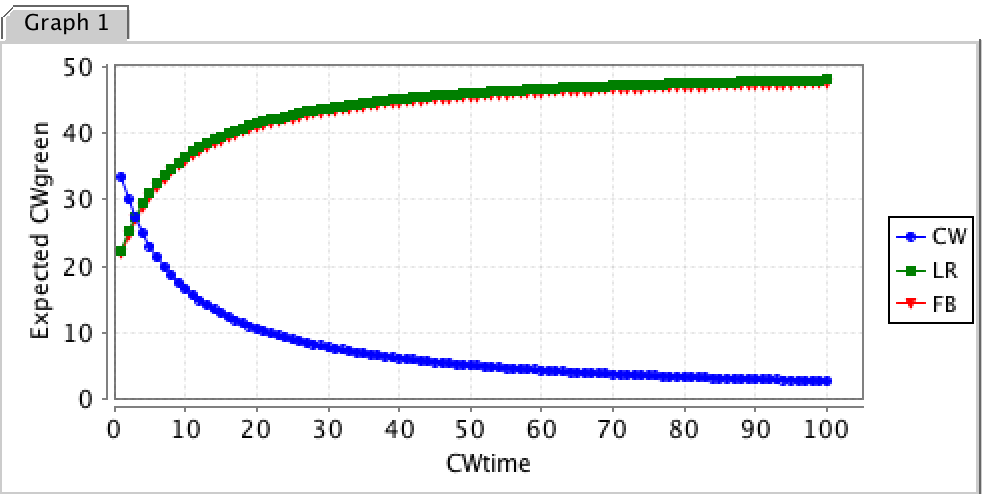
\includegraphics[width=0.5\textwidth]{picture/graphprism.png}
    \caption{Percentage of green lights between the traffic lights}
\end{figure}

\paragraph{Crosswalk and buses}

Here we obtain more specific details about our implementation. For example, we calculate the effect of the time that has elapsed between two buses with as constant the time of a pedestrian call. We also look at the effect of the time between two pedestrians on the green light of the bus for different time between two buses. \\

We choose to have only one dependent variable for each of the graph and fixed the value of the independent variable.
\begin{itemize}
	\item FB : the light for the car in the north-south direction,
	\item LR : the light for the car in the east-west direction,
	\item CW : the light for the pedestrians,
	\item BUS : the light for the bus.
\end{itemize}


\begin{figure}[H]\label{fig:cwfirst}
  \centering
    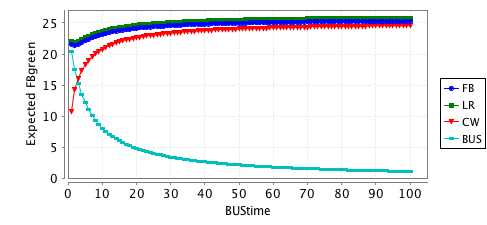
\includegraphics[width=0.5\textwidth]{picture/CWtime1.png}
    \caption{Effect of time that has elapsed between two buses with pedestrian call = 1 unit of time}
\end{figure}

\begin{figure}[H]\label{fig:cwthree}
  \centering
    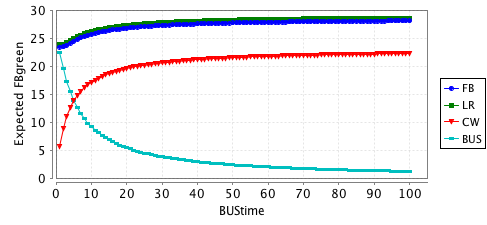
\includegraphics[width=0.5\textwidth]{picture/CWtime3.png}
    \caption{Effect of time that has elapsed between two buses with pedestrian call = 3 units of time}
\end{figure}

\begin{figure}[H]\label{fig:busbus}
  \centering
    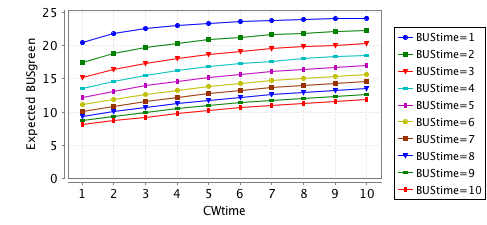
\includegraphics[width=0.5\textwidth]{picture/CWtimeOnBUS.png}
    \caption{Effect of the time between two pedestrians calls on the bus green light}
\end{figure}

Those details can be seen on Figure 4.4, 4.5 and 4.6.